\subsection{Zoom: Column-Based Lists}
The next step identified by \cite{Shneiderman1996} is to zoom in order to explore areas of interest. Upon clicking on the clusters presented in the overview, CubanSea opens a new window and displaying the result list as depicted in figure \ref{fig:zoom:piracy}. The content of a cluster is displayed similar to a regular result list. This is intentional in order for users to feel more comfortable working with it. The primary difference is that instead of a pagination, a dynamically growing column-based list is used. The total result list is displayed split into multiple columns using a fixed height. Result overflow is handled by adding additional columns, thus changing the scrolling direction from horizontal to vertical. This technique allows users to simultaneously percieve a high number of result items and is based on traditional layouts common in file browsers such as the Windows Explorer and Nautilus. Consequetly, viewers are largely familiar with this visualization and intuitively work with it.

Instead of requiring the user to issue a ``go to next page'' command, the interface continously fetches additional results from the server and adds them to the list, while allowing the user to simultaneously work with those results already fetched. As a result, the user can navigate through the result space more quickly, simply by scrolling to the right and left. Potentionally all results can be viewed within one single interface. The downside to this technique is the continuous server load. As long as results are available, requests are issued fetching these results. Traditional pagination interfaces only fetch specifically requested resources. For this application, in consideration of increasing hardware and network performance and due to its experimental nature, this downside is acceptable. Future scalability could be easily achieved by evaluating the users scroll behaviour, requesting new results only as the user reaches the end of the currently displayed list and thus implicitly requests additional results.

\begin{figure*}[!t]
	\centering
	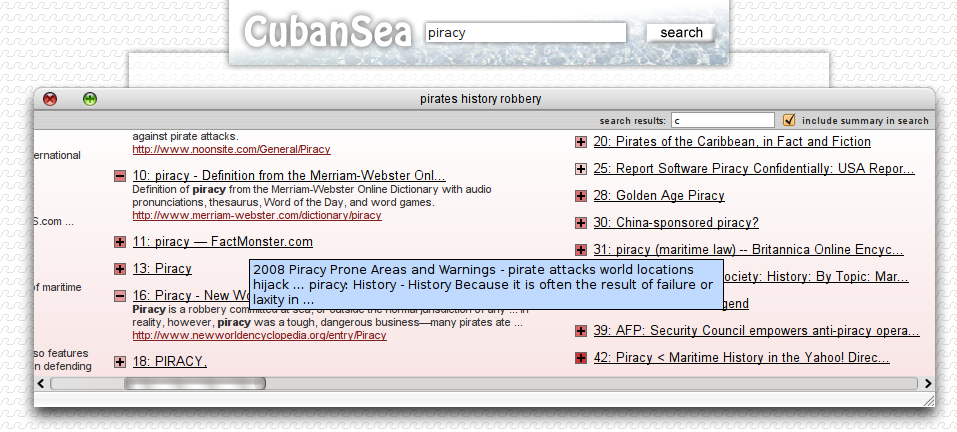
\includegraphics[width=6.5in]{cubansea-details_piracy}
	\caption{Using the mouse-over tooltip functionality for displaying the snippet}
	\label{fig:details:piracy}
\end{figure*}

The column-based result list is enriched with small squares encoding the relevance of the result to the cluster as discussed in \cite{Hoeber2006a}. However, instead of using a color scale comprised by distinct colors, the primary color assigned to the cluster is used and its opacity is set to the relative membership value. The relative membership value is the membership value of the specific result divided by the highest membership in the cluster. This way a continuous scale from 0.0 to 1.0 is achieved with 1.0 being the hightest membership, thus being most relevant to the cluster. By using the opacity, the squares of relevant results have a higher contrast than those of results less important. Hence, they stick out more \cite{Ware2004}. Consequently, the more relevant a result is for a cluster, the more attention it attracts with its square, hereby aiding the user in identifying interesting results. In order to enhance the perception of differences between high rated results, the relative membership is taken to the second power.